\documentclass[border=5mm]{standalone}
\usepackage{tikz}
\usetikzlibrary{calc, intersections, arrows}


\begin{document}
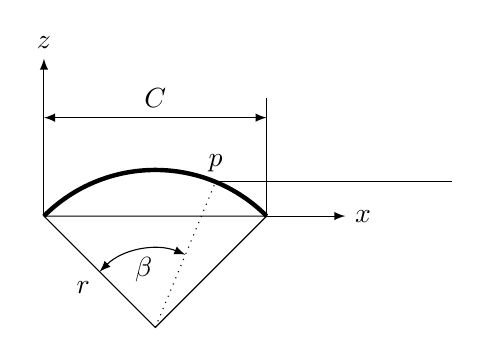
\begin{tikzpicture}
\tikzset{>=latex}
\newcommand{\tikzAngleOfLine}{\tikz@AngleOfLine}
  \def\tikz@AngleOfLine(#1)(#2)#3{%
  \pgfmathanglebetweenpoints{%
    \pgfpointanchor{#1}{center}}{%
    \pgfpointanchor{#2}{center}}
  \pgfmathsetmacro{#3}{\pgfmathresult}%
  }

  \coordinate (o) at (0,0);
  \coordinate (c) at ($(o)+(-45:2)$);
  \coordinate (e) at ($(c)+(45:2)$);
  \coordinate (t) at ($(c)+(67.5:2)$);
  \coordinate (p) at ($(c)+(67.5,2)$);
  \coordinate (m) at ($(o)!0.5!(e)$);
  \coordinate (c1) at ($(o)+(0,1.5)$);
  \coordinate (c2) at ($(e)+(0,1.5)$);
  \coordinate (c3) at ($(e)+(0,1.25)$);
  \coordinate (m2) at ($(t)+(3,0)$);

    \tikzAngleOfLine(c)(o){\AngleStart}
    \tikzAngleOfLine(c)(t){\AngleEnd}
    \draw[<->] (c)+(\AngleStart:1cm) arc (\AngleStart:\AngleEnd:1 cm);
    \node at ($(c)+({(\AngleStart+\AngleEnd)/2}:0.75 cm)$) {$\beta$};

    \draw[thin] (o) -- node[below left] {$r$} (c) -- (e) -- cycle;
    \draw [ultra thick] (o) arc (135:45:2);
    \draw[thin,->] (e) -- +(1,0) node[right] {$x$};
    \draw[thin,->] (o) -- (0,2) node [above] {$z$};
    %\draw[thick,->] (m) -- (t) node[above] {$z_c$};
    %\draw[thick,->] (o) -- node[above right=0.05] {$x_c$} (m);
    \draw[thin, dotted] (c) -- (t) node[above] {$p$};
    \draw[thin] (e) -- (c2);
    \draw[thin,<->] (0,1.25) -- node[above] {$C$}(c3);
    \draw[thin] (t) -- (m2);
    %\draw[thin,<->] ($(e)+(0.5,0)$)-- node[left] {$t$} +($(t)-(m)$);
\end{tikzpicture}
\end{document}

